%%=====================================================================
%% VERSION 2 (post-SBESC 2026 revision; #33972 rejected on 2026-09-24).
%% IEEE two-column conference template. The submitted version is kept
%% untouched in ../artigo/. Reviewer -> change map: RASTREABILIDADE-REVISOES.md
%% New results (bands, single learners, weights, nested CV, attack rate,
%% fixed generator, evasion): ../experimentos-revisao.py ->
%% ../artefatos-modelos/experimentos-revisao.json
%%=====================================================================
\documentclass[conference]{IEEEtran}
\IEEEoverridecommandlockouts

\usepackage{cite}
\usepackage{amsmath,amssymb,amsfonts}
\usepackage{graphicx}
\usepackage{booktabs}
\usepackage{array}
\usepackage{tikz}
\usetikzlibrary{positioning,arrows.meta}
\usepackage[hidelinks]{hyperref}
\usepackage{url}
\usepackage{balance} % balances the two columns on the last page (avoids trailing blank space)
\def\BibTeX{{\rm B\kern-.05em{\sc i\kern-.025em b}\kern-.08em T\kern-.1667em\lower.7ex\hbox{E}\kern-.125emX}}

\begin{document}

\title{Autonomous Contextual Authentication for Web\\ Applications Combining an AI Ensemble and\\ Permissioned Blockchain Auditing}

\author{\IEEEauthorblockN{Jo\~ao Guedes de Brito}
\IEEEauthorblockA{\textit{Graduate Program in Systems and Products Engineering (PPGESP)}\\
\textit{Instituto Federal da Bahia (IFBA)}\\
Salvador, Bahia, Brazil \\
joaoguedesdebrito@gmail.com}
\and
\IEEEauthorblockN{Cleber Jorge Lira de Santana}
\IEEEauthorblockA{\textit{Graduate Program in Systems and Products Engineering (PPGESP)}\\
\textit{Instituto Federal da Bahia (IFBA)}\\
Salvador, Bahia, Brazil \\
cleberlira@ifba.edu.br}
}

\maketitle

\begin{abstract}
Traditional authentication mechanisms based on static passwords or
fixed multi-factor authentication (MFA) remain widely deployed, yet
they ignore the behavioral and environmental context of each access
attempt and are increasingly exploited by credential stuffing,
phishing, and account-takeover attacks. This paper presents an
autonomous contextual authentication system for web applications that
combines a machine-learning ensemble with permissioned-blockchain
auditing. Each login is described by fourteen contextual and
behavioral features, which are scored by an ensemble of Isolation
Forest, Random Forest, and a multilayer neural network; the resulting
risk score drives a three-band adaptive decision (grant, step-up to
MFA, or block). We further propose an audit layer in which each
decision, together with the score and features that justified it, is
recorded on a Hyperledger Fabric ledger, and we discuss when this choice
is warranted over signed logs and append-only databases. At this stage
the audit layer is a design: the prototype stores decisions in a
relational database and the Fabric integration has not been carried out,
so no immutability property is claimed. In an \emph{offline} evaluation
on a synthetic dataset of 50{,}000 login records (95\% legitimate, 5\% suspicious), the ensemble
reached 98.1\% accuracy, 80.2\% F1-score, and a 0.99 ROC-AUC on a
held-out test set, with a 0.8\% false-positive rate at the selected
binary threshold and an inference latency of roughly 33\,ms per request;
with the three bands, 7.3\% of attacks pass unchallenged and 2.7\% of
legitimate accesses face friction. The ensemble beats every single
learner by about 3 F1 points, but an attacker who merely mimics timing
features cuts recall from 77.6\% to 50.7\%, and to 18.0\% with a
residential proxy.
Labels come from the synthetic generator itself; the results therefore
characterize the feasibility of the pipeline, not expected production
performance.
\end{abstract}

\begin{IEEEkeywords}
contextual authentication, risk-based authentication, machine
learning, ensemble, anomaly detection, blockchain, audit trail,
information security.
\end{IEEEkeywords}

\section{Introduction}
Authentication is the first line of defense of web applications.
Historically it has relied on a knowledge factor---the
password---whose weaknesses are well documented: passwords are reused
across services, leaked at scale, and exploited through brute force,
credential stuffing, and phishing~\cite{nist80063b,verizon2024}.
Multi-factor authentication (MFA) mitigates part of this exposure by
combining knowledge, possession, and inherence factors, but static MFA
still falls to social engineering, SIM swapping, and real-time code
interception, while adding friction to the user
experience~\cite{nist80063b}.

The scale of the problem justifies moving beyond the credential alone.
Credential stuffing, phishing, and the use of stolen credentials remain
among the leading vectors in breach reports, and account-takeover fraud
imposes direct financial and reputational costs on organizations and
end users~\cite{verizon2024}. Password reuse turns any single leak into
a cross-service liability, while commoditized attack tooling makes
large-scale login abuse cheap and highly automated. Crucially, static
defenses---password-strength policies and one-time codes---do not
observe \emph{how}, \emph{when}, or \emph{from where} a login occurs,
and therefore cannot distinguish a legitimate user from an adversary who
already holds valid credentials. Regulatory frameworks such as the
Brazilian LGPD~\cite{lgpd2018} add a further requirement: automated
access decisions over personal data must be demonstrably accountable.
Together, these pressures motivate authentication decisions that are
conditioned on the full context of each attempt---and that leave a
verifiable trail of \emph{why} each decision was taken.

To address these limitations, the NIST digital identity
guidelines and the Zero Trust model recommend \emph{adaptive}
mechanisms, in which the level of verification required is proportional
to the estimated risk of each attempt~\cite{nist80063b,rose2020}. This
shifts authentication from a binary, static decision toward a
continuous, context-sensitive assessment---an approach known in the
literature as risk-based authentication (RBA). Empirical studies of
production services show, however, that deployed RBA is dominated by a
single signal (typically the IP address) and by hand-tuned
heuristics~\cite{wiefling2019,wiefling2023}. In parallel, when access
decisions are delegated to autonomous models, they must be
\emph{auditable} by third parties (e.g., for regulatory compliance), a
requirement that decision logs held by a single operator do not fully
satisfy.

This paper proposes an autonomous contextual authentication system
that couples an adaptive machine-learning (ML) decision to its audit
record. The main contributions are:
\begin{itemize}
  \item an end-to-end architecture that fuses fourteen contextual and
        behavioral features into a single risk score computed by an
        ensemble of Isolation Forest, Random Forest, and a neural
        network, driving a three-band adaptive decision;
  \item the design of a permissioned-blockchain audit layer coupled to
        the decision, with an explicit justification of \emph{when} a
        blockchain is needed over signed logs or append-only databases,
        and a statement of what the current prototype does not yet
        implement; and
  \item a reproducible \emph{offline} evaluation of the risk engine on
        synthetic data (code, data, models, and hyperparameters
        published).
\end{itemize}

The remainder of the paper is organized as follows. Section~\ref{sec:related}
reviews related work. Section~\ref{sec:arch} describes the proposed
architecture, Section~\ref{sec:ai} the AI decision engine, and
Section~\ref{sec:bc} the blockchain audit layer.
Section~\ref{sec:method} presents the evaluation methodology and
Section~\ref{sec:results} the results. Section~\ref{sec:conclusion}
concludes.

\section{Related Work}
\label{sec:related}
\textbf{Behavioral biometrics.} Continuous authentication from
interaction patterns is well established. TypeNet~\cite{acien2022} and
TypeFormer~\cite{stragapede2024} identify users from keystroke dynamics
with low error rates, and Touchalytics~\cite{frank2013} shows that
touchscreen patterns discriminate users on mobile devices. These works
confirm the discriminative power of user behavior but focus on a
single biometric modality and do not address immutable auditing of the
decisions. Contemporary surveys of sensor-based continuous
authentication~\cite{abuhamad2021} corroborate that behavioral signals
generalize across many modalities, while highlighting open challenges in
robustness, template ageing, and real-world deployment---challenges that
argue for fusing behavior with other contextual signals rather than
relying on a single modality.

\textbf{Contextual and device signals.} Beyond behavior, the device and
network context of a login is itself discriminative. Alaca and van
Oorschot~\cite{alaca2016} classify twenty-nine device-fingerprinting
methods for augmenting web authentication and compare them by stability,
spoofing difficulty, and distinguishability, and Andriamilanto \emph{et
al.}~\cite{andriamilanto2021} show, on more than four million browsers,
that browser fingerprints carry enough distinctiveness and stability to
strengthen authentication. Freeman \emph{et al.}~\cite{freeman2016}
introduced the first public probabilistic model that scores a login as
normal or suspicious from signals such as source IP, geolocation,
browser configuration, and time of day. These works validate individual
contextual signals but treat them largely in isolation and do not couple
the resulting decision to a tamper-evident record.

\textbf{Risk-based authentication.} Wiefling \emph{et
al.}~\cite{wiefling2019} conducted the first large-scale empirical
study of RBA in the wild, and later work~\cite{wiefling2023} showed
that risk factors must be carefully tuned per service. Our proposal
follows this line but replaces fixed heuristics---and the single-signal,
statistically-scored models that preceded them~\cite{freeman2016}---with
a multi-signal ML ensemble, and adds a non-repudiation layer.

\textbf{Anomaly detection.} Isolation Forest~\cite{liu2008} is a
reference for unsupervised outlier detection in high-dimensional
spaces, and supervised and deep models~\cite{goodfellow2016} complement
it when labels are available; Killourhy and Maxion~\cite{killourhy2009}
established a methodological benchmark for keystroke anomaly detection.
We combine both natures---unsupervised and supervised---in an ensemble.

\textbf{Blockchain for auditing.} Although blockchain-based log
auditing has been investigated, most approaches treat event recording
as \emph{decoupled} from the decision mechanism. Systems such as
BlockAudit~\cite{blockaudit} demonstrate scalable, tamper-evident audit
logs on a blockchain, but the logged events originate in applications
external to the recording layer, so the record attests \emph{that} an
event occurred without binding it to the reasoning that produced it. The
intended distinguishing feature of this work is to integrate, in a single flow,
the adaptive AI decision and its immutable record on a permissioned
ledger, so that each stored entry carries the very features and score
that justified the action.
Table~\ref{tab:related} summarizes representative work: no single line
of research simultaneously provides (i)~fusion of multiple contextual
and behavioral signals, (ii)~an adaptive ensemble decision, and
(iii)~audit immutability coupled to the decision.

\begin{table}[t]
\caption{Positioning Against Representative Related Work}
\label{tab:related}
\centering
\footnotesize
\setlength{\tabcolsep}{3.5pt}
\renewcommand{\arraystretch}{1.2}
\begin{tabular}{@{}p{1.85cm}p{1.3cm}ccc@{}}
\toprule
\textbf{Work} & \textbf{Signals} & \textbf{Adapt.} & \textbf{Audit} & \textbf{Data} \\
\midrule
TypeNet~\cite{acien2022} & Keystroke & \checkmark & --- & Real \\
Touchalytics~\cite{frank2013} & Touch & \checkmark & --- & Real \\
Freeman~\cite{freeman2016} & IP/geo/UA & Part. & --- & Real \\
Alaca~\cite{alaca2016} & Device fp. & --- & --- & --- \\
Andriam.~\cite{andriamilanto2021} & Browser fp. & --- & --- & Real \\
RBA~\cite{wiefling2019} & IP/context & Part. & --- & Real \\
Iso.\ Forest~\cite{liu2008} & Generic & Unsup. & --- & --- \\
BlockAudit~\cite{blockaudit} & Log events & --- & \checkmark & --- \\
\textbf{This work} & \textbf{14 ctx.+beh.} & \textbf{Ens.} & \textbf{Des.} & Synth. \\
\bottomrule
\end{tabular}

\vspace{2pt}
{\footnotesize \emph{Adapt.}: adaptive/learned decision (Part.: partial;
Ens.: ensemble). \emph{Audit}: immutable audit coupled to the decision
(Des.: designed, not yet implemented).}
\end{table}

\section{Proposed Architecture}
\label{sec:arch}
The architecture articulates microservices, federated identity
management, AI-based risk analysis, and immutable blockchain recording,
following the principles of security by design and continuous
verification of Zero Trust~\cite{rose2020,nist80053r5}. Rather than a
binary decision at login time, the model adopts a continuous,
risk-oriented perspective. It is organized in five integrated layers
(Fig.~\ref{fig:arch}):

\begin{enumerate}
  \item \textbf{Modular Application.} Independent services (Spring
        Boot) and an Angular front end exposing authenticated REST APIs.
  \item \textbf{Identity and Access.} Federated authentication through
        Keycloak (OAuth2 / OpenID Connect), JWT issuance, and MFA
        support.
  \item \textbf{Contextual Intelligence.} Extraction of the fourteen
        behavioral features and computation of the risk score by the
        ensemble.
  \item \textbf{Adaptive Decision.} Application of the risk thresholds,
        resulting in \emph{grant}, \emph{step-up to MFA}, or
        \emph{block}.
  \item \textbf{Immutable Registry and Audit.} Persistence of each
        decision on a permissioned blockchain, ensuring traceability
        and non-repudiation.
\end{enumerate}

The operational flow is a chained decision pipeline: a login attempt
triggers extraction of the contextual features; the AI engine computes
the risk score; the decision thresholds are applied; the outcome is
recorded on the blockchain; and the system grants access, requires MFA,
or blocks the attempt. The separation into layers allows each
responsibility to evolve independently and specific security policies
to be enforced at each level.

\textbf{Threat model and design rationale.} The system assumes an
adversary who may already hold valid credentials---obtained through
leakage, phishing, or reuse---and who can attempt logins from arbitrary
networks and devices, but who cannot forge the consensus of the
permissioned ledger nor observe the private state of the risk models.
Under this model the layers address complementary concerns: L2
establishes \emph{who} claims to authenticate, L3 estimates \emph{how
likely} that claim is legitimate given the context, L4 turns the
estimate into a proportionate action, and L5 makes the action
\emph{accountable}. The intermediate band assumes the adversary does
not hold the second factor; an adversary with credentials and access to
the second factor (e.g., through real-time phishing) is contained only by
the block band, which is why the share of attacks falling in each band
must be reported, not just binary performance. Decoupling estimation (L3) from enforcement (L4) is
deliberate: risk thresholds can be re-tuned, and models retrained,
without touching the identity provider, and the audit layer stays
agnostic to the specific learners in use. Because each decision is
written together with its justification---the hash of the input features
and the score that produced it---an auditor can later replay any
decision and verify that the recorded action matches the policy in force
at that time, without having to trust the operator's own logs. This
tight coupling between \emph{deciding} and \emph{recording} is the
property that distinguishes the proposal from pipelines that log events
after, and separately from, the decision.

\textbf{Prototype status.} The architecture above is the design target.
The public prototype (Spring Boot + Angular) currently implements:
password login with its own JWTs (Keycloak integration exists as an
optional configuration profile, not used in the current deployment);
TOTP-based MFA; a Java version of the three learners, trained at start-up;
and persistence of each decision in a relational table (PostgreSQL) with
hash chaining. Three divergences from the text are made explicit:
(i)~the models evaluated in Section~\ref{sec:results} are those of the
\emph{offline} Python pipeline, not the Java prototype, which uses a
different set of fourteen features; (ii)~in the prototype, the ensemble
score is still combined into a trust score
($T = 0.4\,H + 0.3\,(1-A) + 0.2\,R + 0.1\,X$, with $H$ success history,
$A$ AI risk, $R$ recent behavior, and $X$ external factors), and MFA is
required when $T<0.5$, with no block band; (iii)~layer L5 is not
connected to a Fabric network: the corresponding service is a simulator,
and integrity verification of the hash chain is not yet functional.
Aligning the prototype with Eq.~(\ref{eq:ensemble}) and the three bands
is the next implementation step.

\begin{figure}[t]
\centering
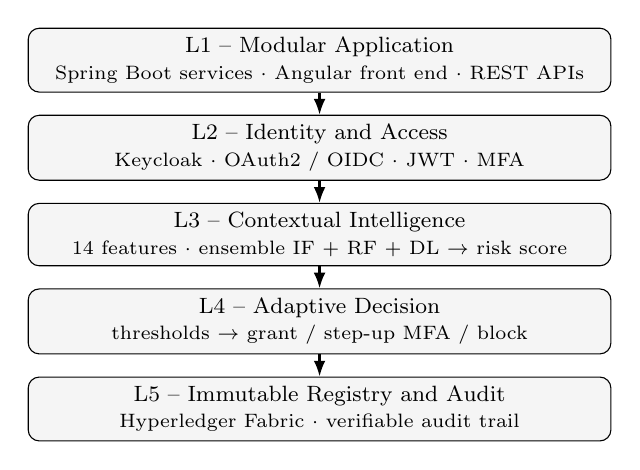
\begin{tikzpicture}[
  layer/.style={draw, rounded corners, minimum width=7.4cm,
    minimum height=0.72cm, align=center, font=\footnotesize, fill=gray!8},
  arr/.style={-{Latex[length=2mm]}, thick}
]
\node[layer] (l1) {L1 -- Modular Application \\ \scriptsize Spring Boot services $\cdot$ Angular front end $\cdot$ REST APIs};
\node[layer, below=0.28cm of l1] (l2) {L2 -- Identity and Access \\ \scriptsize Keycloak $\cdot$ OAuth2 / OIDC $\cdot$ JWT $\cdot$ MFA};
\node[layer, below=0.28cm of l2] (l3) {L3 -- Contextual Intelligence \\ \scriptsize 14 features $\cdot$ ensemble IF + RF + DL $\rightarrow$ risk score};
\node[layer, below=0.28cm of l3] (l4) {L4 -- Adaptive Decision \\ \scriptsize thresholds $\rightarrow$ grant / step-up MFA / block};
\node[layer, below=0.28cm of l4] (l5) {L5 -- Immutable Registry and Audit \\ \scriptsize Hyperledger Fabric $\cdot$ verifiable audit trail};
\draw[arr] (l1) -- (l2);
\draw[arr] (l2) -- (l3);
\draw[arr] (l3) -- (l4);
\draw[arr] (l4) -- (l5);
\end{tikzpicture}
\caption{Five-layer architecture of the proposed system.}
\label{fig:arch}
\end{figure}

\section{AI Decision Engine}
\label{sec:ai}
\textbf{Ensemble.} The risk engine combines three complementary
learners. \emph{Isolation Forest}~\cite{liu2008} acts as the first
level of analysis, isolating outliers in the multidimensional feature
space with few random partitions; it contributes 40\% of the final
weight. \emph{Random Forest} contributes 30\%, capturing non-linear
relations among features while remaining interpretable. A
\emph{multilayer neural network}~\cite{goodfellow2016} contributes the
remaining 30\%, with an input layer of 14 neurons, two hidden layers
(64 and 32 units, ReLU activations, Adam optimizer, no dropout), and a
logistic output. The final score is the weighted average
\begin{equation}
S = 0.4\,S_{\mathrm{IF}} + 0.3\,S_{\mathrm{RF}} + 0.3\,S_{\mathrm{DL}},
\label{eq:ensemble}
\end{equation}
where each component returns a value in $[0,1]$ (0: normal, 1: highly
anomalous). Combining unsupervised and supervised learners aims to
cover both unlabeled novel deviations and known fraud patterns; the
contribution of each learner is measured in Section~\ref{sec:results}.

\textbf{Features.} Each attempt is represented by fourteen features
grouped into four families: \emph{temporal} (access hour, weekday, time since last login, 24\,h access frequency);
\emph{geographic/network} (geodesic distance from the usual location,
network type, ASN, impossible-travel speed); \emph{device/browser}
(browser fingerprint, operating system, device type,
automation/headless detection); and \emph{session behavior} (keystroke
pattern and recent failure history). These signals target credential
stuffing, impossible travel, session hijacking, bots, and
zero-day deviations.

\textbf{Adaptive thresholds.} The score is mapped to three risk bands
whose cut-offs (0.3 and 0.7) are design parameters, not calibrated
values: low risk
($S<0.3$) grants access without additional steps; moderate risk
($0.3\le S<0.7$) triggers MFA; and high risk ($S\ge0.7$) blocks the
attempt, records the event on the blockchain, and notifies the security
administrator. The evaluation in Section~\ref{sec:results} also uses a
single binary threshold ($\tau=0.54$, Section~\ref{sec:method}) that
falls inside the MFA band; precision, recall, and FPR therefore do not by
themselves describe granting or blocking, and per-band performance is
reported separately (Table~\ref{tab:bands}).
The three learners are evaluated sequentially. Periodic retraining
against concept drift~\cite{gama2014} and model versioning are design
requirements not yet implemented.

\section{Blockchain-Based Auditing}
\label{sec:bc}
This section describes the \emph{design} of the audit layer; as stated
in Section~\ref{sec:arch}, it has not yet been integrated with a real
network, and its evaluation is future work. In the design, every decision
is recorded on a permissioned ledger based on
Hyperledger Fabric~\cite{fabric2024}, whose identity control and
structured governance suit corporate and government
environments~\cite{nistir8202}. For each event the ledger stores the
hash of the input features, the risk score, the decision (grant, MFA,
or block), and the transaction timestamp, chained to the previous
record so as to form a chronological chain of evidence.

The choice of a blockchain over simpler mechanisms is justified rather
than assumed. Signed logs and append-only databases already provide
integrity and non-repudiation through cryptographic signatures, and are
sufficient when a single trusted authority operates the registry. The
essential difference of a permissioned blockchain is \emph{not} the
signature itself, but not depending on trust in a single custodian: the
record is replicated and validated by consensus among multiple
participants, becoming resistant to tampering even by privileged
administrators of the system and enabling independent verification by
external auditors. This is decisive here, because access decisions are
made autonomously by AI models and must be auditable by third parties
(e.g., LGPD~\cite{lgpd2018} compliance checks), a scenario in which the
operator alone should not be able to alter the decision trail. We
acknowledge the cost---higher operational complexity and lower
throughput than an append-only store---which is warranted precisely in
multi-party, regulated settings, and delimits the scope in which the
blockchain is actually necessary. This cost has not yet been measured;
the planned evaluation requires a network with at least two
organizations and measures commit latency, throughput under load, and
detection of a deliberate tampering attempt by an administrator of one
organization. Until then, the prototype's relational record remains
under the control of a single custodian---precisely the setting this
section deems insufficient.

\section{Evaluation Methodology}
\label{sec:method}
\textbf{Dataset and labeling.} In the absence of public labeled
datasets for contextual authentication, a synthetic dataset of
50{,}000 login records was built,\footnote{Dataset (labeled CSV, trained models, and metrics): \url{https://github.com/jgbcientista/gestao-autonomo/tree/main/docs/artefatos-modelos}} with a 95\%/5\%
legitimate/suspicious split fixed as a working hypothesis (not a
distribution measured in production). Each record contains the fourteen
features of Section~\ref{sec:ai}. \emph{Each record's label is the
generator branch that produced it} (legitimate or perturbed); there was
no manual review by specialists. All distributions are constants chosen
by the authors to represent plausible corporate usage, not parameters
estimated from real data: the access hour is a Gaussian ($\mu=13$\,h,
$\sigma=3.2$\,h) truncated to $[0,23]$---treated as a linear variable,
without circular encoding---, the inter-login interval is exponential,
the 24-hour frequency Poisson, and the geodesic distance half-normal;
the browser-fingerprint and keystroke-similarity scores are high-mean
Gaussians truncated to $[0,1]$, and the device, operating-system, ASN,
and network-type indicators are categorical variables with frequencies
fixed in the generator. Suspicious records are obtained by perturbing
\emph{two to four} randomly chosen features of a legitimate profile into
anomalous ranges (late-night hour, weekend, login burst, impossible
distance and travel speed, atypical network or ASN, unknown operating
system or device, diverging fingerprint and keystroke, automation, recent
failures). About 5\% of the legitimate records receive a perturbation in
\emph{one} feature, drawn \emph{from the same ranges} used for the
attacks; this choice is what produces the false positives. Finally,
Gaussian noise with standard deviation $0.30$ times the column's
standard deviation is added to every feature. Because the noise is also
applied to categorical and non-negative variables, the dataset contains
physically implausible values (e.g., ASN $=0.94$ or negative travel
speed); we report this generator limitation rather than hide it, and
fixing it is part of future work. Because the data are synthetic, no
personally identifiable information is collected at this stage; the move
to real data will follow the minimization and anonymization principles
required by the LGPD~\cite{lgpd2018}.

\textbf{Protocol.} The dataset was split in a stratified way into 70\%
training and 30\% testing. The scaler (standardization) and the min-max
normalization of the Isolation-Forest score are fitted on the training
split only. Hyperparameters (Table~\ref{tab:hyper}) were fixed
\emph{a priori}, with no search; the only tuned parameter is the decision
threshold, chosen on the grid $\{0.20, 0.21, \dots, 0.80\}$ as the value
maximizing training F1 ($\tau=0.54$) and applied unchanged to the test
set. To estimate variability, a stratified 5-fold cross-validation was
run \emph{on the training split only}, refitting the scaler, the models,
and the threshold inside each fold; the test split takes no part.
Performance was measured by precision, recall, F1-score, false-positive
rate (FPR), ROC-AUC, area under the precision-recall curve (PR-AUC, more
informative under imbalance), and inference latency. For the three-band
decision we define the \emph{friction rate} (share of legitimate accesses
that receive MFA or are blocked) and the \emph{silent-pass rate} (share of
attacks granted with no challenge). Random seeds were fixed.

\textbf{Additional analyses.} With the same pipeline we also evaluate:
(i)~each learner alone, with its own threshold chosen on the training
split; (ii)~all 66 weight combinations on a 0.1 grid (a sensitivity
analysis, not a selection); (iii)~attack rates of 1\%, 2\%, 5\%, 10\%, and
20\%; (iv)~a generator variant with no noise on categorical and count
features and with non-negative continuous features clipped, which removes
the implausible values; and (v)~an attacker who knows the fourteen
features and replaces the ones it controls with values drawn from the
legitimate distribution, at four cumulative levels: timing and attempt
rate; network, ASN, and location (residential proxy near the victim);
fingerprint, OS, device, and automation (anti-detect browser); and
keystroke pattern.
To support independent verification, the
source code, the trained-model artifacts, and the scripts that generate
the dataset and reproduce every experiment are openly
available.\footnote{\url{https://github.com/jgbcientista/gestao-autonomo}}

\textbf{Reproducibility.} A single entry-point script regenerates the
entire pipeline deterministically from the fixed seed: the labeled
dataset (50{,}000 rows with the fourteen features and the class label),
the three trained learners together with the feature scaler (serialized
with \texttt{joblib}), the ensemble configuration (component weights,
the Isolation-Forest score-normalization bounds, and the decision
threshold selected by the best training-set F1), and a machine-readable
metrics file holding every figure reported in
Section~\ref{sec:results}. Re-executing the script on a clean
environment reproduces the reported metrics; different scikit-learn
versions change only the third decimal place (e.g., F1 from 0.802 to
0.805), so that a reviewer can audit the whole pipeline end to end---from raw
feature generation to the final decision threshold---without access to
any private or personally identifiable data. This packaging is what
turns the ``about 50{,}000 records'' description into an artifact that a
third party can regenerate, inspect, and extend.

\begin{table}[t]
\caption{Hyperparameters (fixed a priori)}
\label{tab:hyper}
\centering
\footnotesize
\setlength{\tabcolsep}{3pt}
\renewcommand{\arraystretch}{1.15}
\begin{tabular}{@{}p{1.9cm}p{6.0cm}@{}}
\toprule
\textbf{Component} & \textbf{Configuration} \\
\midrule
Pre-processing & standardization (z-score) fitted on training split \\
Isolation Forest & 100 trees; contamination 0.05; score $-$\texttt{score\_samples}, min-max normalized on training split and clipped to $[0,1]$ \\
Random Forest & 120 trees; unlimited depth; \texttt{class\_weight=balanced} \\
Neural net (MLP) & hidden layers 64--32, ReLU, Adam, 220 iterations, no dropout; logistic output \\
Ensemble & $0.4\,S_{\mathrm{IF}}+0.3\,S_{\mathrm{RF}}+0.3\,S_{\mathrm{DL}}$ \\
Threshold & grid 0.20--0.80 (step 0.01), max.\ training F1 $\Rightarrow\tau=0.54$ \\
Data & 50{,}000 records; 5\% suspicious; noise $0.30\sigma$; seed 42 \\
\bottomrule
\end{tabular}
\end{table}

\textbf{Baselines.} Table~\ref{tab:baseline} contrasts the proposal
with representative baselines from the literature and practice. The
baseline figures are taken from the cited literature and were not
re-executed here; the comparison is therefore qualitative regarding the
capabilities of each approach. The three comparison axes are not
arbitrary; they follow from the requirements that the literature places
on modern authentication. \emph{Context-awareness} (Ctx.) reflects the
NIST and Zero-Trust prescription that verification be conditioned on the
signals of each attempt rather than on the credential alone
\cite{nist80063b,rose2020}, and is the property that empirical studies
of risk-based authentication find decisive in the
wild~\cite{wiefling2019,freeman2016}. \emph{Adaptivity} (Adapt.)
captures whether the response is proportional to the estimated
risk---the core principle of risk-based
authentication~\cite{nist80063b,wiefling2019,wiefling2023}---rather than
a fixed, one-size-fits-all rule. \emph{Auditability} (Audit.) addresses
the accountability of automated decisions over personal data, a
requirement made explicit by data-protection regulation such as the
LGPD~\cite{lgpd2018} and, more broadly, by the need for independent
verification when access is delegated to autonomous models. Together
these axes span the two properties a contextual-authentication system
must jointly satisfy---deciding correctly and being verifiable---while
the \emph{main limitation} column indicates where each baseline falls
short on at least one of them.

\begin{table}[t]
\caption{Comparison With Reference Approaches}
\label{tab:baseline}
\centering
\footnotesize
\setlength{\tabcolsep}{3.5pt}
\renewcommand{\arraystretch}{1.2}
\begin{tabular}{@{}p{1.7cm}cccp{2.05cm}@{}}
\toprule
\textbf{Approach} & \textbf{Ctx.} & \textbf{Adapt.} & \textbf{Audit.} & \textbf{Main limitation} \\
\midrule
Password + static 2FA & --- & --- & --- & Ignores context; phishing/SIM swap \\
IP-based RBA~\cite{wiefling2019} & Part. & Heur. & --- & Single feature; manual tuning \\
Statistical scoring~\cite{freeman2016} & \checkmark & Stat. & --- & Few signals; no decision audit \\
Keystroke only~\cite{killourhy2009} & \checkmark & --- & --- & Offline, single factor (EER $\approx$9.6\%) \\
\textbf{Proposed} & \textbf{\checkmark} & \textbf{Ens.} & \textbf{Des.} & Synthetic data; audit still a design \\
\bottomrule
\end{tabular}

\vspace{2pt}
{\footnotesize \emph{Ctx.}: uses login context; \emph{Adapt.}: adaptive
decision (Heur.: heuristic; Stat.: statistical; Ens.: ensemble);
\emph{Audit.}: immutable audit coupled to the decision (Des.: designed).}
\end{table}

\section{Results and Discussion}
\label{sec:results}
On the held-out test set (30\% of the data, unseen during training) the
ensemble reached an accuracy of 98.1\%, precision of 83.0\%, and recall
of 77.6\% for suspicious accesses, with an F1-score of 80.2\% and a
ROC-AUC of 0.99, indicating strong ranking capability between
legitimate and suspicious accesses. The false-positive rate remained
low at 0.8\%, which is relevant to usability. Cross-validation restricted
to the training split confirms the order of magnitude (F1
$80.3\%\pm1.3\%$; AUC $0.990\pm0.002$), with thresholds between 0.42 and
0.56 depending on the fold. The test confusion matrix is
TN\,=\,14{,}131, FP\,=\,119, FN\,=\,168, TP\,=\,582.
Table~\ref{tab:results} summarizes these figures.

\begin{table}[t]
\caption{Ensemble Performance on the Held-Out Test Set}
\label{tab:results}
\centering
\renewcommand{\arraystretch}{1.2}
\begin{tabular}{@{}lc@{\hspace{6mm}}lc@{}}
\toprule
\textbf{Metric} & \textbf{Value} & \textbf{Metric} & \textbf{Value} \\
\midrule
Accuracy   & 98.1\% & F1-score       & 80.2\% \\
Precision  & 83.0\% & ROC-AUC        & 0.99   \\
Recall     & 77.6\% & False-pos.\ rate & 0.8\% \\
\midrule
\multicolumn{2}{@{}l}{F1 (5-fold CV, training)} & \multicolumn{2}{l}{$80.3\%\pm1.3\%$} \\
\multicolumn{2}{@{}l}{AUC (5-fold CV, training)} & \multicolumn{2}{l}{$0.990\pm0.002$} \\
\multicolumn{2}{@{}l}{Ensemble latency (\emph{offline})} & \multicolumn{2}{l}{$\approx$33\,ms/request} \\
\bottomrule
\end{tabular}
\end{table}

\textbf{Three-band decision.} Table~\ref{tab:bands} applies the 0.3/0.7
bands to the test scores. Among legitimate accesses, 97.3\% are granted
without challenge (2.7\% friction rate) and only 0.1\% are blocked. Among
attacks, 62.5\% are blocked, 30.1\% receive MFA, and 7.3\% pass silently.
Since the MFA band only stops an adversary lacking the second factor
(Section~\ref{sec:arch}), the effective protection against one holding
credentials and second factor is the blocked share, not binary recall.

\begin{table}[t]
\caption{Three-Band Decision on the Test Set}
\label{tab:bands}
\centering
\footnotesize
\renewcommand{\arraystretch}{1.15}
\begin{tabular}{@{}lccc@{}}
\toprule
\textbf{True class} & \textbf{Grant} & \textbf{MFA} & \textbf{Block} \\
 & ($S<0.3$) & & ($S\ge0.7$) \\
\midrule
Legitimate & 97.3\% & 2.6\% & 0.1\% \\
Suspicious & 7.3\% & 30.1\% & 62.5\% \\
\midrule
\multicolumn{4}{@{}l}{Friction rate: 2.7\% \quad Silent-pass rate: 7.3\%} \\
\bottomrule
\end{tabular}
\end{table}

\textbf{Contribution of each learner.} Table~\ref{tab:single} compares the
ensemble with each learner trained alone in the same pipeline. The
ensemble gains about 3 F1 points over the best single learner (0.802
versus 0.775 for the Random Forest), lowers the FPR from 1.15\% to 0.84\%,
and raises PR-AUC from 0.86 to 0.90. The 0.4/0.3/0.3 weights, however,
were not optimized: over the 66 combinations evaluated, test F1 ranges
from 0.767 (Isolation Forest only) to 0.820, and the adopted setting
ranks 19th. The best combinations give 0.6--0.8 to the Isolation Forest
and little or no weight to the neural network. Choosing weights from this
result would fit the test set; proper selection on a validation split is
left to the next stage.

\begin{table}[t]
\caption{Ensemble Versus Single Learners (Test)}
\label{tab:single}
\centering
\footnotesize
\setlength{\tabcolsep}{4pt}
\renewcommand{\arraystretch}{1.15}
\begin{tabular}{@{}lcccccc@{}}
\toprule
\textbf{Model} & $\tau$ & \textbf{Prec.} & \textbf{Rec.} & \textbf{F1} & \textbf{FPR} & \textbf{PR-AUC} \\
\midrule
Isolation Forest & 0.45 & 0.763 & 0.772 & 0.767 & 1.26\% & 0.855 \\
Random Forest    & 0.60 & 0.779 & 0.771 & 0.775 & 1.15\% & 0.857 \\
Neural network   & 0.48 & 0.757 & 0.792 & 0.774 & 1.34\% & 0.860 \\
\textbf{Ensemble} & 0.54 & \textbf{0.830} & 0.776 & \textbf{0.802} & \textbf{0.84\%} & \textbf{0.903} \\
\bottomrule
\end{tabular}
\end{table}

\textbf{Sensitivity to attack rate and to the generator.}
Table~\ref{tab:prop} repeats the experiment for other attack rates. AUC
stays at 0.99, but prevalence-dependent metrics change markedly: with 1\%
attacks, F1 drops to 0.63 and the silent-pass rate rises to 24.0\%,
because the Isolation Forest (contamination equal to the attack rate) and
the F1-selected threshold come to favour the majority class. In
production, where attacks tend to be rarer than 5\%, this is the relevant
scenario. Fixing the generator noise (item~(iv) of the additional
analyses) barely changes the results (F1 0.809, AUC 0.992, silent pass
6.9\%), indicating that the implausible values did not inflate the
metrics.

\begin{table}[t]
\caption{Sensitivity to the Attack Rate}
\label{tab:prop}
\centering
\footnotesize
\setlength{\tabcolsep}{4pt}
\renewcommand{\arraystretch}{1.15}
\begin{tabular}{@{}lccccc@{}}
\toprule
\textbf{Attacks} & \textbf{F1} & \textbf{AUC} & \textbf{PR-AUC} & \textbf{Friction} & \textbf{Silent pass} \\
\midrule
1\%  & 0.632 & 0.989 & 0.718 & 0.8\% & 24.0\% \\
2\%  & 0.720 & 0.991 & 0.809 & 1.1\% & 16.7\% \\
5\%  & 0.802 & 0.992 & 0.903 & 2.7\% & 7.3\% \\
10\% & 0.869 & 0.992 & 0.944 & 3.1\% & 6.4\% \\
20\% & 0.917 & 0.993 & 0.976 & 4.2\% & 3.7\% \\
\bottomrule
\end{tabular}
\end{table}

\textbf{Adversarial evasion.} Table~\ref{tab:evasion} shows the effect of
an attacker who knows the features. Mimicking only the timing and rate of
attempts---a trivial step---already cuts recall from 77.6\% to 50.7\% and
raises the silent-pass rate from 7.3\% to 28.4\%. With a residential proxy
near the victim, recall falls to 18.0\% and 64.4\% of attacks pass
unchallenged; with an anti-detect browser, practically all pass. This is
partly a consequence of the generator: synthetic attacks \emph{are
defined} as deviations in these features, so removing them erases the
signal. But it also exposes a real limit of the approach: most of the
fourteen features are attacker-controllable, and only the keystroke
pattern and the account history resist an informed attacker.
Hard-to-forge features and evasion defenses are therefore a requirement,
not a refinement.

\begin{table}[t]
\caption{Evasion by an Attacker Who Knows the Features (Test Attacks)}
\label{tab:evasion}
\centering
\footnotesize
\setlength{\tabcolsep}{3pt}
\renewcommand{\arraystretch}{1.15}
\begin{tabular}{@{}p{3.3cm}cccc@{}}
\toprule
\textbf{Features mimicked (cumulative)} & \textbf{Recall} & \textbf{Grant} & \textbf{MFA} & \textbf{Block} \\
\midrule
None & 77.6\% & 7.3\% & 30.1\% & 62.5\% \\
+ timing and rate & 50.7\% & 28.4\% & 33.1\% & 38.5\% \\
+ network, ASN, location (proxy) & 18.0\% & 64.4\% & 25.3\% & 10.3\% \\
+ fingerprint, OS, device, automation & 2.9\% & 91.1\% & 8.0\% & 0.9\% \\
+ keystroke (all) & 0.3\% & 98.1\% & 1.9\% & 0.0\% \\
\bottomrule
\end{tabular}

\vspace{2pt}
{\footnotesize Recall at the binary threshold $\tau=0.54$; other columns use the 0.3/0.7 bands.}
\end{table}

Latency was measured only in the \emph{offline} pipeline (scikit-learn,
one sample per call, median of 300 calls): 4.0\,ms for the Isolation
Forest, 29.2\,ms for the Random Forest, and 0.05\,ms for the neural
network, executed sequentially, for a total of about 33\,ms---a
machine-dependent figure dominated by the Random Forest. The latency of
the complete login flow, the cost of audit recording, and throughput were
not measured; these figures depend on the integration described in
Section~\ref{sec:bc} and are left to the next stage.

\textbf{Discussion.} The partial results are promising and suggest the
technical feasibility of the approach; however, because they stem from
synthetic data and a preliminary stage, they do not yet allow the
central hypothesis to be confirmed conclusively. A rigorous comparison
against the baselines and validation with real data remain necessary
before any quantitative claim of superiority. Even so, in a
controlled environment the ensemble separated perturbed from legitimate
records with an AUC of 0.99, indicating that the chosen features carry
signal when attacks manifest in the ranges modelled by the generator---a
caveat that the evasion analysis makes concrete. No
claim about tamper resistance is made in this version, since the audit
layer has not been evaluated.

\textbf{Error analysis and trade-offs.} The decision threshold is not
fixed a priori but selected as the value that maximizes the F1-score on
the training partition, which makes the operating point explicit and
tunable per deployment: lowering it raises recall at the cost of more
step-up challenges, whereas raising it favours a frictionless experience
at the risk of missing borderline attacks. At the chosen point the
confusion matrix on the test set is dominated by true negatives, and the
residual errors concentrate on the boundary between mildly anomalous
legitimate accesses and low-intensity suspicious ones---exactly the
region the noise model was designed to make ambiguous. This explains
both the sub-90\% F1 and the low false-positive rate: the ensemble is
conservative, preferring an occasional missed detection over penalizing
legitimate users, a bias that is appropriate for an authentication
front-end where usability friction carries a direct business cost. The
three learners contribute complementary views---the Isolation Forest
flags globally rare feature combinations without labels, while the
Random Forest and the neural network exploit the labeled decision
boundary. We deliberately refrain from reading these
figures as evidence of superiority over the baselines of
Table~\ref{tab:baseline}: the baselines were not re-executed on the same
data, and the synthetic generator, however carefully calibrated, cannot
capture the full adversarial diversity of production traffic. These
observations frame the experiment as a feasibility study whose next step
is validation on real, non-repudiable logs collected under the very
architecture proposed here.

\textbf{Limitations and threats to validity.} Four limitations bound
the reach of our conclusions. First, external validity is constrained by
the use of synthetic data: although the generative process reproduces
plausible corporate-usage distributions, it captures neither the long
tail of atypical yet legitimate behavior nor the adversarial creativity
observed in real traffic, so the reported metrics should be read as an
optimistic upper bound rather than as expected production performance.
Second, construct validity depends on heuristic labeling: because the
labels derive from the same rules that describe the fraud patterns, they
may introduce a circularity in which the ensemble re-learns the
boundaries encoded in the generator itself---a risk that only labeling
over real, analyst-reviewed incidents fully removes. Third, the
comparison against the baselines is deliberately qualitative, as they
were not re-executed on the same dataset; quantitative claims of
superiority therefore remain outside the scope of this preliminary
phase. Fourth, adversarial robustness is low: as
Table~\ref{tab:evasion} shows, most features can be mimicked by an
informed attacker. We partially mitigate these threats by fixing random
seeds, publishing the hyperparameters, and openly releasing the code and
artifacts for independent inspection; full mitigation, however, requires
collecting real logs under the proposed architecture---a record that
the audit layer, once implemented, should make verifiable---closing the
loop between methodological evaluation and actual
system operation.

\section{Conclusion and Future Work}
\label{sec:conclusion}
This paper presented an autonomous contextual authentication system
that combines an adaptive AI decision with the design of a
permissioned-blockchain audit. The contributions are the architecture
fusing fourteen contextual and behavioral signals through an ensemble,
the design of the decision-coupled audit layer with an explicit
justification for the use of blockchain, and a reproducible
\emph{offline} evaluation of the risk engine. Preliminary experiments on
synthetic data indicated technical feasibility (98.1\% accuracy, 80.2\%
F1-score, 0.99 AUC, $\approx$33\,ms inference latency; 7.3\% silent pass
with the three bands), and the ensemble outperformed every single learner;
the evasion analysis, however, shows that most features are controllable
by an informed attacker. This constitutes a methodological validation rather than a substitute for evaluation on
real data. The immediate next step is to integrate a real Fabric
network with at least two organizations, measuring commit latency,
throughput, and tamper detection, and to align the prototype with
Eq.~(\ref{eq:ensemble}) and the three bands. Further future work includes replacing the synthetic dataset with
real or semi-real data collected in a controlled environment, selecting
weights and thresholds on a validation split, adding hard-to-forge
features and evasion defenses, assessing performance and scalability
under realistic load, and deepening the security analysis against the
threat model. We further plan to investigate the explainability of the
ensemble decisions---exposing, for each block or MFA challenge, the
criteria that contribute most to the risk score---to evaluate system
behavior under prolonged concept drift and adversarial evasion attacks,
and to conduct a usability study that quantifies the friction perceived
by legitimate users when facing adaptive challenges. On the audit side,
we intend to measure the consensus cost of the permissioned network
under realistic login rates and to evaluate periodic anchoring
strategies that preserve independent verifiability without compromising
throughput. We also plan to extend the ensemble with online learning so
that model updates track behavioral drift continuously, and to study calibration techniques
that keep the risk score aligned with the empirical probability of
compromise as the operating environment evolves. Finally, integrating
the proposed decision-and-audit pipeline with a federated identity
deployment at institutional scale would let us assess the end-to-end
latency budget, the operational overhead of key and certificate
management, and the governance model required for multiple organizations
to jointly operate and audit the permissioned ledger. Taken together,
these directions aim to progressively close the gap between the
controlled feasibility study reported here and a production-grade
deployment whose adaptive decisions remain, at every step, both
effective and independently verifiable.

\balance
\begin{thebibliography}{00}
\bibitem{nist80063b} National Institute of Standards and Technology, ``Digital Identity Guidelines: Authentication and Lifecycle Management,'' NIST SP 800-63B, 2017.
\bibitem{verizon2024} Verizon, ``2024 Data Breach Investigations Report (DBIR),'' Verizon Business, 2024.
\bibitem{rose2020} S. Rose, O. Borchert, S. Mitchell, and S. Connelly, ``Zero Trust Architecture,'' NIST SP 800-207, 2020.
\bibitem{wiefling2019} S. Wiefling, L. Lo Iacono, and M. D\"urmuth, ``Is This Really You? An Empirical Study on Risk-Based Authentication Applied in the Wild,'' in \emph{IFIP SEC}, 2019, pp. 134--148.
\bibitem{wiefling2023} S. Wiefling, P. R. J\o rgensen, S. Thunem, and L. Lo Iacono, ``Pump Up Password Security! Evaluating and Enhancing Risk-Based Authentication on a Real-World Large-Scale Online Service,'' \emph{ACM Trans. Priv. Secur.}, vol. 26, no. 1, 2023.
\bibitem{freeman2016} D. Freeman, S. Jain, M. D\"urmuth, B. Biggio, and G. Giacinto, ``Who Are You? A Statistical Approach to Measuring User Authenticity,'' in \emph{Proc. Netw. Distrib. Syst. Secur. Symp. (NDSS)}, 2016.
\bibitem{alaca2016} F. Alaca and P. C. van Oorschot, ``Device Fingerprinting for Augmenting Web Authentication: Classification and Analysis of Methods,'' in \emph{Proc. 32nd Annu. Comput. Secur. Appl. Conf. (ACSAC)}, 2016, pp. 289--301.
\bibitem{andriamilanto2021} N. Andriamilanto, T. Allard, G. Le Guelvouit, and A. Garel, ``A Large-scale Empirical Analysis of Browser Fingerprints Properties for Web Authentication,'' \emph{ACM Trans. Web}, vol. 16, no. 1, pp. 1--62, 2021.
\bibitem{abuhamad2021} M. Abuhamad, A. Abusnaina, D. Nyang, and D. Mohaisen, ``Sensor-Based Continuous Authentication of Smartphones' Users Using Behavioral Biometrics: A Contemporary Survey,'' \emph{IEEE Internet Things J.}, vol. 8, no. 1, pp. 65--84, 2021.
\bibitem{blockaudit} A. Ahmad, M. Saad, and A. Mohaisen, ``Secure and Transparent Audit Logs with BlockAudit,'' \emph{J. Netw. Comput. Appl.}, vol. 145, art.\ 102406, 2019.
\bibitem{acien2022} A. Acien, A. Morales, R. Vera-Rodriguez, J. Fierrez, and J. V. Monaco, ``TypeNet: Deep Learning Keystroke Biometrics,'' \emph{IEEE Trans. Biom. Behav. Identity Sci.}, vol. 4, no. 1, pp. 57--70, 2022.
\bibitem{stragapede2024} G. Stragapede, P. Delgado-Santos, R. Tolosana, R. Vera-Rodriguez, R. Guest, and A. Morales, ``TypeFormer: Transformers for Mobile Keystroke Biometrics,'' \emph{Neural Comput. Appl.}, vol. 36, pp. 18531--18545, 2024.
\bibitem{frank2013} M. Frank, R. Biedert, E. Ma, I. Martinovic, and D. Song, ``Touchalytics: On the Applicability of Touchscreen Input as a Behavioral Biometric for Continuous Authentication,'' \emph{IEEE Trans. Inf. Forensics Security}, vol. 8, no. 1, pp. 136--148, 2013.
\bibitem{liu2008} F. T. Liu, K. M. Ting, and Z.-H. Zhou, ``Isolation Forest,'' in \emph{IEEE Int. Conf. Data Mining (ICDM)}, 2008, pp. 413--422.
\bibitem{killourhy2009} K. S. Killourhy and R. A. Maxion, ``Comparing Anomaly-Detection Algorithms for Keystroke Dynamics,'' in \emph{IEEE/IFIP DSN}, 2009, pp. 125--134.
\bibitem{goodfellow2016} I. Goodfellow, Y. Bengio, and A. Courville, \emph{Deep Learning}. Cambridge, MA: MIT Press, 2016.
\bibitem{gama2014} J. Gama, I. \v{Z}liobait\.e, A. Bifet, M. Pechenizkiy, and A. Bouchachia, ``A Survey on Concept Drift Adaptation,'' \emph{ACM Comput. Surv.}, vol. 46, no. 4, pp. 1--37, 2014.
\bibitem{fabric2024} Hyperledger Foundation, ``Hyperledger Fabric Documentation, v2.5,'' Linux Foundation, 2024.
\bibitem{nistir8202} National Institute of Standards and Technology, ``Blockchain Technology Overview,'' NISTIR 8202, 2018.
\bibitem{nist80053r5} National Institute of Standards and Technology, ``Security and Privacy Controls for Information Systems and Organizations,'' NIST SP 800-53 Rev.\ 5, 2020.
\bibitem{lgpd2018} Brazil, ``Lei n.\ 13.709/2018 -- Lei Geral de Prote\c{c}\~ao de Dados Pessoais (LGPD),'' 2018.
\end{thebibliography}

\end{document}
